\chapter{Implementierung}\label{ch:implementierung}
%Eigene Arbeiten
%Jetzt kommt der spannende Teil! Ihre eigene Arbeit wird hier ausführlich dargelegt. Dieses Kapitel ist kein Protokoll ihrer Studienarbeit, sondern eine Darlegung der entwickelten Verfahren. Die Detailtiefe sollte derart sein, dass es anderen möglich, ist die dargestellten Verfahren sowohl nachvollziehen als auch zu implementieren. Implementierungsdetails können im Bedarfsfall auftauchen, sollten aber eventuell in einen Appendix ausgelagert werden. Versuchen Sie zu vermeiden, dieses Kapitel mit dem nächsten zu vereinen. Die Verfahrensbeschreibung und die Evaluation sollten in den meisten Fällen getrennt sein.

%Es lassen sich auch mehrere Bilder nebeneinander platzieren wie z.B. in Abbildung
%\ref{fig:multipic} zu sehen ist.
%\begin{figure}[hpbt]
% \centering
%  %%----start of first subfigure----
%  \subfloat[FIFO size limited to 20 entries]{
%   \label{fig:multipic:a} %% label for first subfigure
%   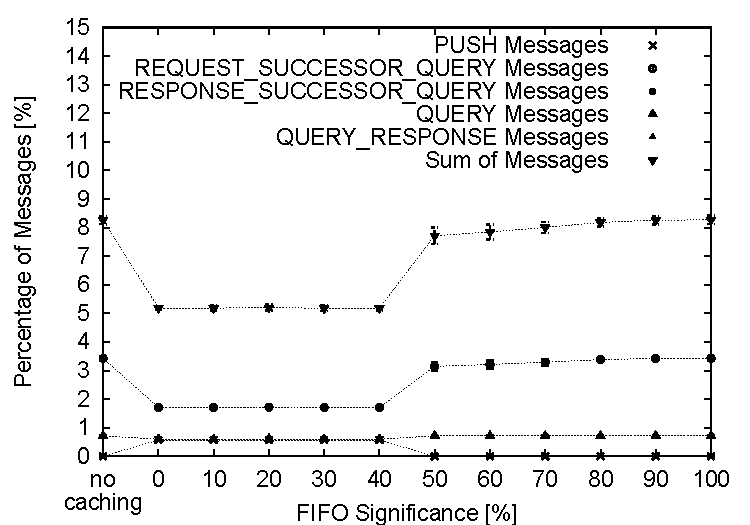
\includegraphics[width=0.48\linewidth]{pic1}}
%  \hspace{0.01\textwidth}
%  %%----start of second subfigure----
%  \subfloat[FIFO size limited to 30 entries]{
%   \label{fig:multipic:b} %% label for second subfigure
%   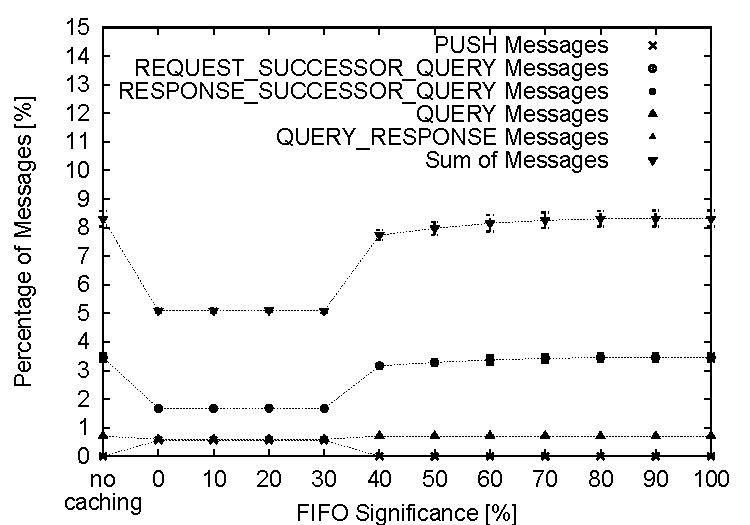
\includegraphics[width=0.48\linewidth]{pic2}}\\[0pt] % horizontal break
%  %%----start of third subfigure----
%  \subfloat[FIFO size limited to 40 entries]{
%   \label{fig:multipic:c} %% label for third subfigure
%   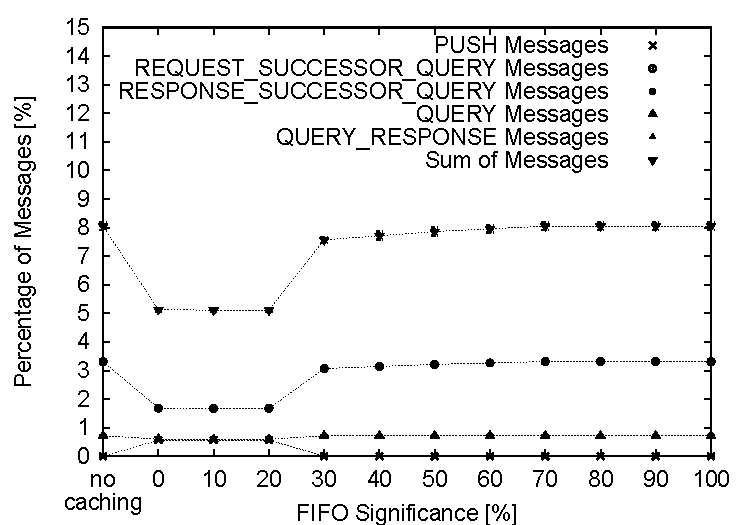
\includegraphics[width=0.48\linewidth]{pic3}}
%  \hspace{0.01\textwidth}
%  %%----start of fourth subfigure----
%  \subfloat[FIFO size limited to 50 entries]{
%   \label{fig:multipic:d} %% label for fourth subfigure
%   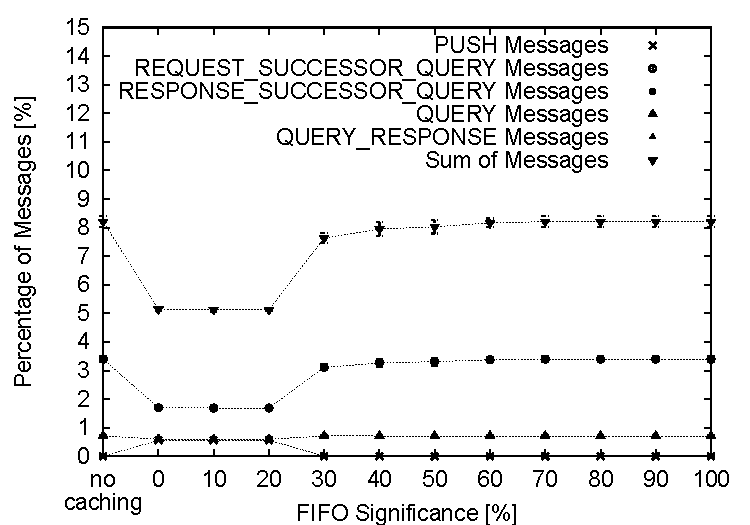
\includegraphics[width=0.48\linewidth]{pic4}}
% \caption[Observed message fractions and 95\% confidence intervals for Chord]{Observed message fractions and 95\% confidence intervals for Chord without the influence of churn. The FIFO capacity varies from 20 (\ref{fig:multipic:a}) -- 50 (\ref{fig:multipic:d}) entries (decadic steps).}
% \label{fig:multipic} %% label for entire figure
%\end{figure}
%
%\subsection{Programm Code}
%Eine elegante Möglichkeit, Programmtext einzubinden, lässt sich mit dem listings-Paket erreichen.
%Das \verb|HelloWorld| Programm aus Listing \ref{lst:hw} hat in Zeile \ref{line:hw3} übrigens einen Programmierfehler.
%\begin{lstlisting}[float=htp,caption=Hello World,label=lst:hw,language=Java, numbers=left, numberstyle=\tiny, stepnumber=2, numbersep=8pt, escapeinside={//@}{@//},backgroundcolor=\color{yellow},xleftmargin=3ex,xrightmargin=1ex]
%public class HelloWorld {
%    public static void main(String[] args) {
%        Syste.out.println("Hello, World"); //@\label{line:hw3}@//
%    }
%}
%\end{lstlisting}

